%% background

%  a. introduction

Geometry reconstruction has drawn a lot of attention in the computer vision community (\Hartley2003, \Seitz2006, and \Prince2012). The goal is to reconstruct the three dimensional structure of a particular scene given the data, usually multiple images (Multi-View Stereo). The images can come from different cameras (unordered set), or from the same camera (sequence) that potentially has been moved around. For many algorithms the relative locations from the cameras are required. They are either obtained by calibration between the different cameras or images (\eg by some identifiable pattern visible in all the images, or measured using external sensors), or estimated based on features naturally occurring in the images. When the positions are known, all the pixels in an image are known to be a projection from a particular point somewhere on a line through the camera centre and the pixel on the image plane, with the location of the point on the line being the only ambiguity. The next task now is to estimate the geometry of the scene pictured in those images, given this ambiguous information. Different approaches exist to tackle this problem, of which we will discuss four categories: layers (Section \ref{layers}), space carving (Section \ref{carving}), structure from motion (Section \ref{sfm}), and Multi-View Stereo using Depth Maps (Section \ref{mvs}). We like to note, however, that often multiple approaches are combined and overlap exist. Not all the techniques being discussed are directly relevant to the proposed algorithm, but they give a sense of the variety of approaches being published and try to give a general overview of the geometry reconstruction research literature.


%  b. Layers in video
\pagebreak
\section{Layers in Video}  \label{layers}
One of the earlier, and in some aspects simpler, attempts to represent geometry in images is the use of layers. Images are assumed to be a composition of multiple, possibly overlapping, surfaces that can move relative to one another from frame to frame in a sequence. Objects pictured in images can be at different distances to the camera, resulting in overlapping surfaces when projected onto an image (\ie captured). Successfully identifying coherent surfaces, including their mutual occlusions and movements from one frame to another, allows for a scene representation consisting of \emph{layers}. Such a representation usually consists of one background layer plus one or more foreground layers representing objects moving in front of the background layer.

As one of the first to suggest representing sequences of images with layers, \Wang1994 decomposed images into `motion layers' by analysing the motion of extracted segments in the subsequent images using optical flow. Segments with similar motions are combined, and grown and depth-ordered by tracking them over the sequence, resulting in more extensive layers. The layers can then be used in combination with estimated simple motion models to reconstruct the sequence in a memory-efficient way. Multiple extensions on this scheme exist. For example, \Jojic2001 subdivided layers into flexible sprites that can vary their shapes according to a probabilistic model. The sprites and their probabilistic models are learned using the Expectation Maximisation algorithm on a representation consisting of one appearance and one mask pixel vector per sprite. Theoretically, the unsupervised EM learning approach even allows for finding sprites in related but unordered photo collections. Another approach, suggested by \Smith2004, is to extract and track edges over the sequence in order. Motion models are then fit to the edges using the EM algorithm. The edges, which form a better criterion for segment borders than the locally-smoothed optical flow vector field, are used to find a good segmentation of the frames and segments with similar motion models are again merged, thereby resulting in layers.

Although layered representations do have the notion of depth-ordering - and thus occlusion - they do not aim at recovering the exact depth of the layers, and inherently do not reconstruct three-dimensional geometry. In the next section, we move on to three alternative approaches that aim at true geometry recovery.

Layers are relevant for the current work because initially the intuition was raised that footage of an outdoor scene can be segmented into layers by tracking feature points and noticing when occlusions happen. However, for these feature points we can estimate the three-dimensional location by using Structure from Motion techniques (Section \ref{sfm}), allowing to reconstruct more than relative order. Hence, the step from layers to real three-dimensional reconstruction was made and the proposed method as described in Section \ref{method} originated.


%  c. Carving
\pagebreak
\section{Space carving}  \label{carving}
While layers in videos try to represent geometry by their projections onto the image planes, thereby ignoring the original three-dimensional geometrical shapes, space carving aims at estimating the actual surface of objects in a scene. To reconstruct 3D from flat projections, space carving assumes the camera poses are known, \ie we have calibrated cameras. The poses are either known due to explicit calibration (using a calibration object or external sensor), or estimated based on the natural content of the images.

Usually, space carving is based on finding silhouettes \cite{Hartley2003, Matusik2000}, thus segmenting each of the images into a binary background and foreground `layer' or mask. These techniques are also known as Structure from Silhouettes. The pixels in the images are known to be projections of points somewhere on lines from the camera centres passing through the pixels, but the locations on the lines (\ie depths) are unknown. Space carving based on silhouettes\footnote{Part of the literature reserves the term Space Carving for space carving based on photo-consistency as described later on; here, it is used for both photo-consistency and silhouette-based space carving iteratively refining a model represented by a voxel grid.}. does not estimate this depth; instead, it uses the background-foreground masks to categorise each line as either intersecting with an object, or not. The foreground mask therefore represents a cone of space in which the projected object must lie, at unknown distance. 

For reconstruction, usually a 3D volume is chosen that lies in between the camera poses, and the volume is discretised and represented as a \emph{voxel grid} - although polygonal representations have been proposed too. Space carving starts with all the voxels marked as `object'. For each camera pose, all the voxels are projected onto the image plane. Voxels projecting to pixels not set as foreground (\ie onto the background mask) are set to `non-object', finally resulting in the intersection of cones in which the object must lie (see Figure \ref{fig:carving}). This intersection is called \emph{visual hull} or \emph{convex hull}. It can be used as the final reconstruction, or used as a useful prior for further processing as the maximum (convex) boundary in which search can continue.

\begin{figure}[htb!]
 \centering
 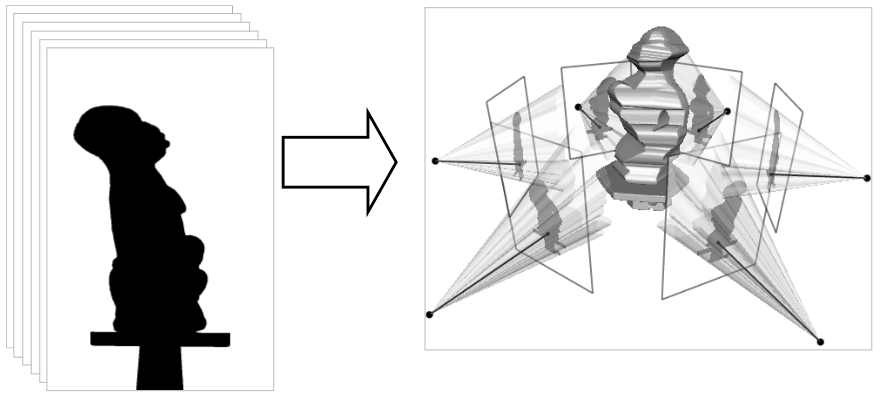
\includegraphics[width=1.0\textwidth]{img/carving}
 \caption{Carving using silhouettes. Image taken from `How to prepare and deliver a presentation' [ppt] by R. Cipolla, who adopted it from unknown source}
 \label{fig:carving}
\end{figure}

Segmenting images in foreground and background masks can be accomplished by a simple threshold, or by learning more advanced colour models for both. This can be user-guided or automated. For example, \Campbell2007 automatically learned foreground colour models using pixels at the centre of the images (requiring the user making the footage to fixate at the object of interest) and background colour models using pixels near the image corners. The initial colour models are used together with the calibrated camera poses to make an initial binary segmentation in a voxel grid. The segmentation is then used to refine the colour models, and the process is repeated until the solution converges. As is common in algorithms involving voxel grid representations, \Campbell2007 use a Markov Random Field (MRF) prior for the segmentation step, promoting local smoothness for obtaining a global solution. A min-cut/max-flow graph-cut algorithm like the one presented by \Boykov2004 is used to find the solution. This process is also known as regularisation.

Using more pictures in the space carving approach will give better approximations. However, concavities are not visible from silhouettes, so they will not turn up in the final reconstruction. The acquired visual hull therefore is only a broad approximation of the object's surface. Space carving is very suitable to do on a turn-table, for which the background model is known and also the relative camera poses are known due to controlled turn-table rotation. However, a turn-table is only feasible for objects small enough to put on the device. Placing a green screen behind objects is also a possibility, resulting in the same easy silhouette segmentation. Green screens have their limits too, making it an unsuitable remedy for outdoor scenes, where the background often is not controllable. Furthermore, space carving is not suitable for dynamic scenes. As a last disadvantage, multiple objects are not easy recognisable in a single silhouette and will result in ghosting objects \cite{Guan2007}.

Extensions have been proposed to overcome the limited applicability of carving based on silhouettes. For example, \GuanOld added time-dependent Bayesian probability to the voxel variables, allowing space carving to be used in dynamic scenes. In their representation, voxels represent probabilities on occlusions before and after the voxel on a line passing through the centres of a set of calibrated cameras, filming from fixed locations. Using time-dependencies, their algorithm is able to follow dynamic objects over time, \eg a human walking through a temple. To find silhouettes, a per-pixel Gaussian background colour model is made for every camera before the dynamic object enters the scene. The estimates of the silhouettes are used as a prior for the next time frame, allowing to spot the object moving behind static occluders. When the object moves extensively through the scene, static occluders will turn up when they occlude the object. Even concavities in static occluders can be detected if an object moves, in fact allowing to carve away all human reachable locations by walking through the scene. In a later publication, \Guan2008 extended their algorithm to detect and label multiple dynamic objects. Each time a new, unknown silhouette (that differs enough from the colour models learned so far) enters the scene, a new appearance colour model is learned. Although the algorithm only works with fixed cameras and dynamic objects, it does have notion of visibility and occlusion.

An alternative to space carving with silhouettes is space carving based on photo-consistency, as introduced by \SeitzOld. Hereby, voxels are projected onto all image planes that are able to see the voxel according to the current voxel grid. The set of pixels a voxel projects to are then checked for photo-consistency in compliance with a reflectance model (BRDF). The photo-consistency check returns the probability of this set of pixel colours originating from the same surface point. For a low photo-consistency score, it is unlikely that this voxel is part of a solid object, and so it is carved away. The process continues until all the remaining uncarved voxels have a high photo-consistency. Although results look promising, the algorithm has some problems with low-textured (\ie uniformly coloured) objects and objects with repetitive textures. Furthermore, the method does not scale very well to bigger environments with lots of same coloured objects, and assumes Lambertian surfaces for all objects. In practise, pixels usually have no unique colour and reflective objects are not uncommon.

% TODO: improve
As a last example in the space carving literature, we discuss the work by \Hernandez2007, who further explored the concept of visibility using the photo-consistency criterion. The algorithm introduced by \SeitzOld is extended to include a probabilistic voxel grid: voxels are not carved one by one, but assigned the photo-consistency probability for being part of the surface of an object \footnote{In fact, a fast depth-map (Section \ref{mvs}) computation is done and photo-consistency is calculated only for locations with 3D points nearby}. A second voxel grid represents the visibility evidence, containing probabilities of voxels being visible by at least one camera. This will give a penalty to voxels that are presumed not to be visible from any camera, and thus not part of the surface of an object. As a final step, graph-cut is used to combine the photo-consistency and visibility voxel grids, obtaining the assumed surface. Note that occlusion is being used, but only to exclude voxels inside objects, not for refining the shape itself.


%  d. Structure from Motion
\section{Structure from Motion}  \label{sfm}
Geometry reconstruction usually involves measurements in the form of images, that is, flat projections of the three-dimensional world at specific locations (and times). If these locations are known, the process of reconstructing the original scene becomes easier. Therefore, much effort has been put in reliable pose estimation. Structure from Motion, as described extensively by \Hartley2003, tries to accomplish this. Structure from Motion (SfM) uses natural features in images in order to estimate the relative translation and rotation between the camera poses of different images. It is based on the intuition that moving your head (motion) and noticing differences of the different views allows for a rough estimation of objects and distances (structure) in a scene.

For SfM techniques, the camera poses are unknown a priori and need to be estimated based for a set of given images. As a first stage, features such as interest (corner) points are found in all images. One of the most popular features is SIFT, as introduced by \Lowe2004. SIFT features are found by searching for maxima in scale-space, constructed with Derivative of Gaussian filters. For the detected locations, a unique SIFT descriptor is constructed based on a histogram of gradient directions of points nearby. SIFT features are scale and rotation invariant and partially intensity and contrast change invariant. Alternative features can be used too, as long as they can be matched uniquely between images. In the second step, the interest points are matched between images using their descriptor. Using the matching pairs between images allows for estimating the relative transformation from one camera to another by satisfying projective geometry constraints (\Prince2012, Ch15-16, \Hartley2003, Ch10-12). For every image pair with estimated transformation, 3D locations of matched interest points can now be estimated by triangulation (Fig. \ref{fig:sfm_triangulate}). The depth ambiguity for \emph{some points} is now eliminated in each image. The image pair point clouds - possibly containing feature points seen in multiple image pairs - can be combined using Bundle Adjustment (\eg, \Wu2011, \Hartley2003, Ch18), which minimises noise and estimation errors in point and camera pose locations and obtains a global solution. The result is a \emph{sparse point cloud} (Fig. \ref{fig:sfm_sparsepointcloud}), camera models (including pose), plus visibility lists with camera-points pairs.
As an example of using alternative features, \Chandraker2009 developed a Structure from Motion system based on lines, arguing that indoor environments and scenes containing much human-made objects usually lack distinctive feature points, but a rich of straight lines. Line geometry constraints are used to estimate camera translation and rotation in a similar way as in the case points are used.

\begin{figure}[htb!]
 \centering
 \subfigure[3D point location estimation by triangulating two matched feature points in a pair of images]{
  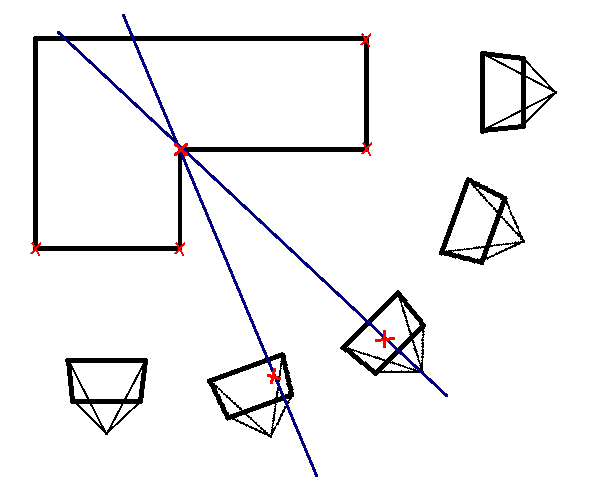
\includegraphics[width=0.45\textwidth]{img/sfm_triangulate}
  \label{fig:sfm_triangulate}
 }
 \subfigure[Sparse point cloud. Image taken from http://grail.cs.washington.edu/rome/dense.html (1st of March 2012)]{
  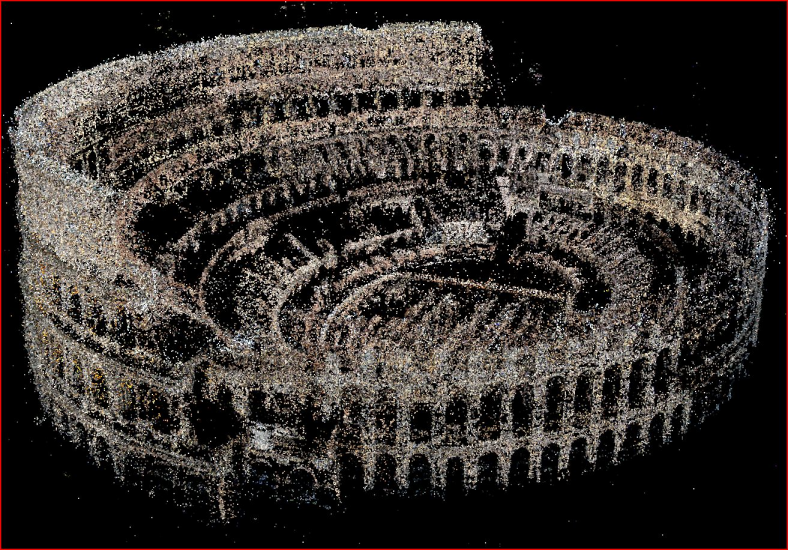
\includegraphics[width=0.45\textwidth]{img/sfm_sparsepointcloud}
          \label{fig:sfm_sparsepointcloud}
 }
 \caption{Structure from Motion}
 \label{fig:sfm}
\end{figure}

After reconstructing both the sparse point cloud and camera poses, usually one of the two is thrown away and the other is used in a subsequent step. Given the sparse point cloud, one can attempt to reconstruct geometry based on the sparse, but reliable points. Different techniques have been used \cite{Seitz2006}. One simple way of doing this is fitting a polygon mesh to the point cloud. More advanced smooth surface fitting is also possible, as has been done for example by Izadi~\etal~\cite{Izadi2011}, but it eliminates strong edges and flat surfaces which are overrepresented in real scenes. Another method is fitting primitive shapes like planes and lines to the point cloud, which works well in human-made environments, but not so well in outdoor scenes. In all cases, assumptions are made on possible interpolation between points close to each other, and lack of texture results in gaps and sometimes missing objects in the reconstruction. In practise, sparse point clouds are rarely used for surface reconstruction. More often, the camera poses are kept and used in combination with the original images using a subsequent algorithm (\eg space carving (Section \ref{carving}) or depth maps (Section \ref{mvs})), obtaining a more dense representation before surface reconstruction is attempted.
% TODO: photo tourism here as possible application of sparse point cloud only


%     - Visibility and Occlusion 
% TODO: move to end MVS? NO: makes sense here
%       (depth maps less clear if they have lists of visibility; plus most papers here are about sparse point clouds)
\subsection{Visibility and Occlusion}
An important observation that did not got a lot of attention in the literature is the fact that the visibility of the points over time (\ie over the image sequence) can not only help selecting and fine-tuning points in either sparse or dense point clouds (as noted in the survey of Seitz~\etal~\cite{Seitz2006} and used in \cite{Merrell2007, Hernandez2007}), but also directly used for surface reconstruction. In other words: occlusion rarely has an essential role in geometry reconstruction. However, visibility tracks over time can help both finding empty space (because we can see points at a certain location from a certain location) and finding occluder objects (because we lost track of a point for a while). Structure from Motion - in addition to pose estimation - therefore does not only deliver sparse points on surfaces, but also gives information about the occupancy state of space between the camera poses and reconstructed sparse points, without the need to find any visual clues at that locations. This observation has an essential role in the proposed approach (Section \ref{method}).

% TODO: improve?
Despite the scarcity of occlusion applications, recently there have been some attempts worth a brief discussion. For example, \ZachOld extent the structure from motion pipeline by an outlier check by using `missing correspondences'. Their method collects triplets of images connected by fair amounts of correspondences. Two of the images are used to triangulate the (sparse) correspondences which are projected into the third image. A probabilistic measure based on the number of found and missing correspondence points in the third image determines whether to discard the third image as a match or not. \Pan2009 propose geometry reconstruction (called ProFORMA) of single, well-textured, objects filmed with a fixed-position camera by calculating a sparse point cloud, converting the point cloud into a mesh using Delaunay tetrahedralisation, and carving away tetrahedra who violate visibility constraints. The carving consists of using intersections of rays from camera poses to points to determine - probabilistically - whether to carve away a intersected tetrahedra, finally obtaining a surface mesh. \Lovi2010 independently developed an almost identical system (called free-space carving) that can be used on more complicated scenes. Both methods use positive visibility information to carve away tetrahedra; however, negative occlusion information is not being used as tetrahedra are assumed to be occupied by default. Furthermore, the tetrahedralisation is based on triangulated feature points, requiring texture to be omnipresent and determinative for quality and resolution of reconstructed models.
Recently \Mcllroy2011 (2011) explored the possible use of both visibility and occlusion information with the aim of constructing high-level scene structure. In their approach, every (sparse) point is assigned a discretised `view sphere' whereby every solid angle bin saves the distance to the furthest camera within the solid angle that detected the point, plus the distance to the closest camera that did not detect the point. Using the view spheres primitives like planes and spheres are fitted to obtain probable locations of scene structure. However, results are shown for simple and well-textured scenes only, modelled by simple planes. Furthermore, since camera poses are used for the fitting, one needs to move extensively through the scene to provide the algorithm with enough camera poses. In contrary, the proposed method (Section \ref{method}) focusses not on the specific camera and point locations but on the rays in between, and thence indirectly finds low-textured and reflective objects using both visibility and occlusion information. In addition, a probabilistic voxel grid is used for discretisation allowing more general shape reconstruction, the implementation is tested on complex real-world scenes, and compared to state-of-the-art Multi-View Stereo results.

%  e. Multi-View Stereo using Depth Maps
\section{Multi-View Stereo using Depth Maps}  \label{mvs}
As a last category of geometry reconstruction methods, we will discuss reconstruction based on dense depth maps, often called stereoscopic. Usually, two steps are involved. In the first step, pairs or bigger sets of images are combined to form dense depth maps. The second step consists of carefully combining the depth maps in order to reconstruct scene geometry globally, for instance - as with SfM - by using bundle adjustment \cite{Wu2011}. Where space carving is mostly defined in scene-space by re-projecting voxel centres onto image planes, multi-view stereo (MVS) using depth maps applies its photo-consistency measure in image-space by comparing pixels \cite{Seitz2006}. Furthermore, as do structure from motion techniques, MVS using depth maps tries to estimate the depth of pixels explicitly. Depth maps, however, try to estimate this depth for every pixel, giving a dense depth or disparity map. However, estimating the depth for every pixel makes it necessary to match with less confidence than possible with SfM points, which can rely on stable and easy comparable feature points such as SIFT. Finally, combining the dense depth maps results in a \emph{dense point cloud}. We will now look into two different ways of creating the depth maps.

%     - active lighting
\subsection{Active lighting}
High precision in solving the depth ambiguity can be reached by actively illuminating part of the scene and searching for the illuminated part in images being taken. Depth map techniques recently received increased interest due to affordable active lighting sensors such as Kinect \cite{Izadi2011} reaching the commercial market, making depth vision suitable for a wider audience, but active lighting systems have been out there for a while. The illumination can consist of some fixed pattern (such as used by the Kinect and exploited by \Izadi2011), a sequence of different patterns (structured light), or a single (laser) point or line that moves over the surface (either for triangulation or time-of-flight). For example, a laser range-finder can be used to accurately map an environment by sending bright laser pulses and measuring travel times. \Huang2000 released a database containing range images obtained this way, together with a statistical analysis of natural depths in images. Although pattern-based devices like Kinect are becoming affordable, their active lighting patterns are weak and hence only suitable for indoor scenes. In general, accurate active lighting devices are less affordable and less practical than omnipresent cheap cameras. Therefore, much research effort has been put into passive depth vision based on regular images pairs.

%     - automated (depth vision)
\subsection{Passive depth vision}

\begin{figure}[htb!]
 \centering
 \subfigure{
  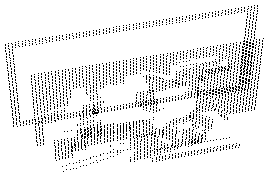
\includegraphics[width=0.45\textwidth]{img/depthmap1}
  \label{fig:depthmap1}
 }
 \subfigure{
  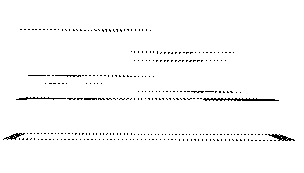
\includegraphics[width=0.45\textwidth]{img/depthmap2}
  \label{fig:depthmap2}
 }
 \caption{Two views of a depth map with few discretised depths, created by graph-cut algorithm. Image taken from own second years project, bachelor artificial intelligence, University of Amsterdam}
 \label{fig:depthmap_layer}
\end{figure}

If one would know, for every pixel in an image, the particular pixel displaying the same point in scene-space in a second image, the relative displacement allows for calculating the distance between that point in space and the camera (\cite{Prince2012}, Ch.14). The depth is estimated by triangulation using displacement and relative camera transformation. Stereoscopic methods often attempt to find pixel pairs or matching patches by using a particular photo-consistency measure and exhaustive search. However, pixel colours are less unique than interest point descriptors and also in general not all the points are visible in both images (occlusion), resulting in ambiguous or missing matches, especially for scenes with low-textured surfaces (\eg painted walls). To simplify the search process, the images are often rectified: morphing them as if they were taken from cameras aligned on a common axis; the search for each pixel now only needs to occur on particular lines of pixels in the second image. Other geometry priors, such as order preservation or minimum and maximum depths, can be used too. Various techniques have been proposed for matching pixels or other primitives in order to obtain smooth depth maps without too many wrong matches or gaps. Hereby, almost all algorithms assume Lambertian surfaces as photo-consistency prior, causing problems for reflective surfaces.

\begin{figure}[htb!]
 \centering
 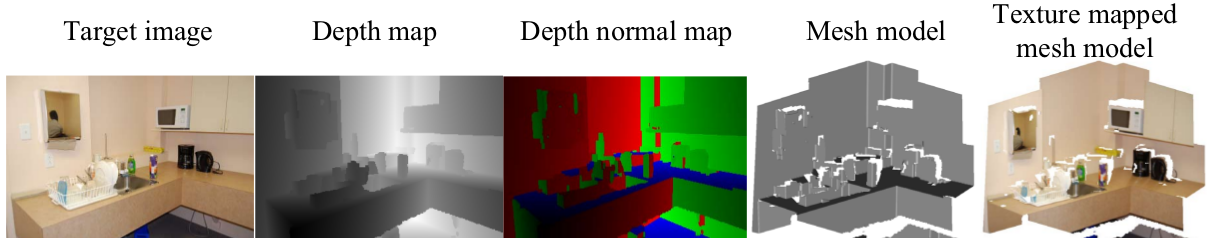
\includegraphics[width=1.0\textwidth]{img/depthmap}
 \caption{Pipeline of \FurukawaOld, including a typical depth map. Images taken from \cite{Furukawa2009}.}
 \label{fig:depthmap}
\end{figure}

Most algorithms are based on matching pixels based on a photo-consistency measure \cite{Seitz2006}. After rectification, only pixels on a particular line need to be tried. Those algorithms often use a prior promoting local smoothness, such as a Markov Random Field (MRF), while using a graph-cut algorithm to find a solution. The number of possible depths can be kept low, lowering the number of computations and increasing smoothness while allowing jumps in depth (\eg Figure \ref{fig:depthmap_layer}). Plane-sweeping algorithms iterate between assigning pixels to planes, and refining the plane equations. One fast but inaccurate plane-sweeping stereo algorithm is used by \Merrell2007 to quickly construct rough depth maps for further processing. Although the depth maps are imprecise, images can be processed very fast and depth maps are merged, obtaining reliable high-resolution dense point clouds. An example using an even stronger planar prior is the work by \FurukawaOld, who search for points with strong confidence depths and normals, and find three dominant axes that are more or less perpendicular. Hypothesis planes are proposed based on the points with strong confidence, and a MRF is used to assign pixels to hypothesis planes, obtaining a planar (Manhattan) world consisting of the most confident planes. Example images from their pipeline are shown in Fig. \ref{fig:depthmap}.

Although planes are a useful prior in indoor scenes and scenes with a lot of human-made architecture, the smoothness prior is more useful in natural environments (\ie general outdoor scenes). The approach of \Hernandez2007 uses photo-consistency in scene-space, whereby projection lines of pixels (\ie a set of possible depth locations) are projected onto camera planes nearby, and the depth candidates giving the best overall photo-consistency are picked. The estimated depths are then used in their carving algorithm using 3D graph-cut on a voxel grid.

Larger areas can be reconstructed using video and reliable location estimation (for example, using SLAM techniques). \Pollefeys2008 developed a system for real-time urban 3D reconstruction. It uses GPS and inertia sensors in addition to image-based pose estimation for reliable localisation, and uses a plane-sweeping dense stereo algorithm with a prior preferring locations containing points from the SfM sparse point cloud. Again, depth maps are created at a high rate and then merged into more accurate models. A similar large-scale reconstruction method is described by \Frahm2010. Building on the success of the Photo Tourism system \cite{Snavely2006} they collect publicly available images on the internet; however, large amounts of images make extensive matching of image pairs intractable, therefore their system finds clusters of images with use of their short image descriptor before structure from motion is applied. For each cluster, dense stereo is used and clusters are merged based on Geo-tag location and inter-connected clusters, finally obtaining a dense reconstruction for a big part of a city, within a day on a powerful PC.

% TODO maybe:
%     - Merging of depth maps (put somewhere logical)
%     - Surface reconstruction (+ multi-res paper)

